% Working IEEE conference paper: evidence-based empirical audit, NOT submission-cleared.
% External StitchingNet scores belong to OLD 182-family-trained models ONLY.
% The NEW 31-photo-inferred model was NOT evaluated on StitchingNet.
\documentclass[conference,a4paper]{IEEEtran}
\usepackage{graphicx,booktabs,array,cite,amsmath,amssymb,url}
\usepackage[hidelinks,pdfauthor={},pdfsubject={Anonymous empirical reproducibility study},pdfkeywords={broken stitch, data leakage, synthetic defects, grouped validation}]{hyperref}
\begin{document}
\title{How Reliable Is Broken-Stitch Classification? An Augmentation-Lineage Audit and Cross-Domain Evaluation}
\author{} % Anonymous manuscript; maintain double-blind review precautions.
\maketitle
\begin{abstract}
Image augmentation can create thousands of stitch-defect examples without adding independent source photographs. We audit an unpublished garment-inspection collection previously associated with 94.91\% reported VGG-16 validation accuracy. Its recovered ZIP contains 7,365 images (7,364 readable). Removing augmentation UUIDs identifies 182 candidate image families, \emph{all} represented in multiple original train/validation/test folders. Filename structure and visual matches further suggest that 151 digitally edited faulty families descend from only 31 normal-photo candidates. On a fresh 21/5/5 inferred-photo-parent split, a fixed ImageNet-pretrained MobileNetV3-Small feature extractor and balanced logistic head obtain 80.20\% accuracy, 0.799 macro-F1 and 74.85\% faulty recall on 1,086 initially held-out augmented images from five candidate source photographs. Separately, an \emph{earlier}, differently trained MobileNet reaches 0.635 macro-F1 and only 57.79\% broken-stitch recall on 3,637 real StitchingNet normal/broken images, with no external tuning. The two tests involve \emph{different} frozen checkpoints and must not be conflated. These observations expose a gap between nominal validation scores and credible defect-screening evidence. Since original photographed-source lineage has not been independently authenticated, our grouped results remain exploratory rather than validated factory generalization.
\end{abstract}
\begin{IEEEkeywords}
broken stitch detection, augmentation leakage, source-grouped evaluation, MobileNetV3, synthetic-to-real transfer, reproducibility
\end{IEEEkeywords}

\section{Introduction}
A broken seam stitch is a small interruption in a repeated, often low-contrast thread pattern. Its appearance changes with fabric, camera distance, lighting and thread colour. Deep classifiers and pretrained features are appealing in garment inspection, but defect collections are frequently enlarged by digital editing and geometrical augmentation. The corresponding image count is then a poor proxy for the number of independent garment or photographic sources. Grouping transformations by the wrong unit can cause related images to occur in training and testing, making apparent generalization misleading.

An unpublished 2022 thesis evaluated activation functions, filters, a CNN, VGG-16 and neural-network ensembles for correct-versus-faulty stitches, reporting a final 94.91\% \emph{validation} accuracy. Its original source code and trained checkpoint are unavailable; the present investigation is a new, non-identical PyTorch reconstruction. The central contribution of this paper is \emph{not} an improved architecture, but a reproducibility audit of image lineage and deliberately qualified empirical evidence on grouped internal and separate external evaluation.

Three questions guide the study: \emph{RQ1}: did the original data folders divide augmentation families across partitions? \emph{RQ2}: what happens when normal images and their likely Photoshop-faulty derivatives share a candidate photo-parent group? \emph{RQ3}: how do strictly frozen models trained on this small synthetic collection perform on genuine sewing-stitch data in another acquisition domain? Importantly, the new inferred-photo-grouped model and the first externally tested model are different runs. The underlying photo-parent relationships remain inferred rather than independently authenticated.

\section{Related Work}
Early textile inspection employed handcrafted texture features and image analysis~\cite{ngan}. Kim \emph{et al.} combined CNN feature maps and image processing for sewing broken-stitch detection~\cite{kim}; Chowdhury \emph{et al.} compared CNN, VGG-16 and VGG-19 on 500 stitch images~\cite{chowdhury}. These precedents mean that adding a pretrained VGG model is not, by itself, a novel contribution. The StitchingNet publication~\cite{stitchingnet} introduced 14,565 sewing-stitch images spanning normal and ten defect types across 11 fabric/thread configurations, enabling more demanding tests of transfer. More recent sewing-image research studies anomaly-based inference~\cite{patchcore2026} and localized segmentation~\cite{stitchingnetseg2026}. The latter derives from StitchingNet, and hence cannot serve as an \emph{independent second} external test after that source has been evaluated.

Compared with these studies, our narrower binary task probes a data-accounting question: whether nominally large augmented datasets really support independent-source accuracy claims. Differences in camera, defect definition, splits, task and score preclude direct performance rankings between published systems.

\section{Data and Audit Procedure}
\subsection{Historical collection and recovered archive}
The thesis describes 31 correct images and roughly 150 digitally modified faulty images, with some images obtained from garment sites and the internet. Because photo capture identity and editing history are incomplete, these figures are \emph{not} 181 verified independent photographs. The recovered 2,146,784,353-byte ZIP contains 7,365 image records (2,734 labelled \texttt{actual}, 4,631 \texttt{faulty}), of which 7,364 decode at $400\times400$ pixels; one normal PNG is unreadable. The 151 named faulty candidate families do not exactly reconcile with the approximately 150 faults described in the thesis.

\begin{figure}[!t]\centering
\begin{minipage}{.48\columnwidth}\centering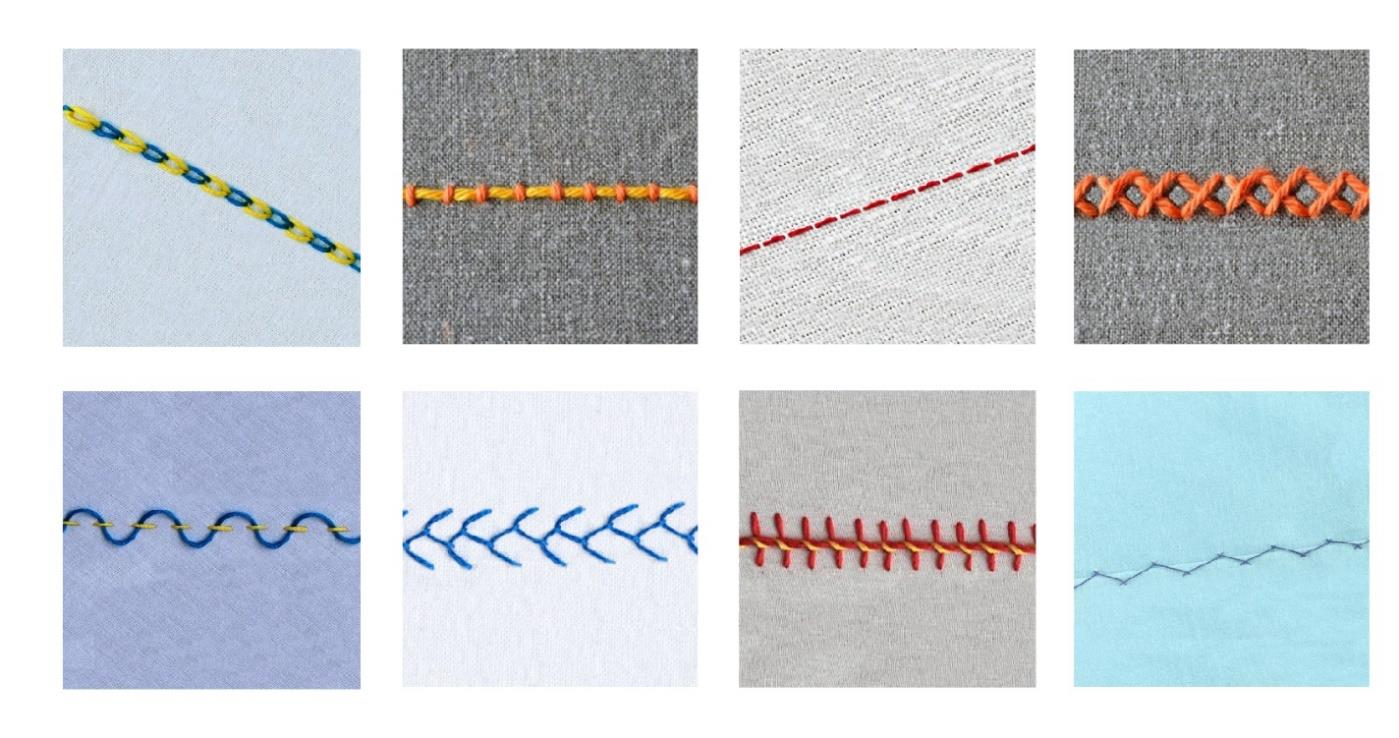
\includegraphics[width=\linewidth]{figures/page33_image1.jpeg}\\[-1mm]{\scriptsize (a) Historical normal example}\end{minipage}\hfill
\begin{minipage}{.48\columnwidth}\centering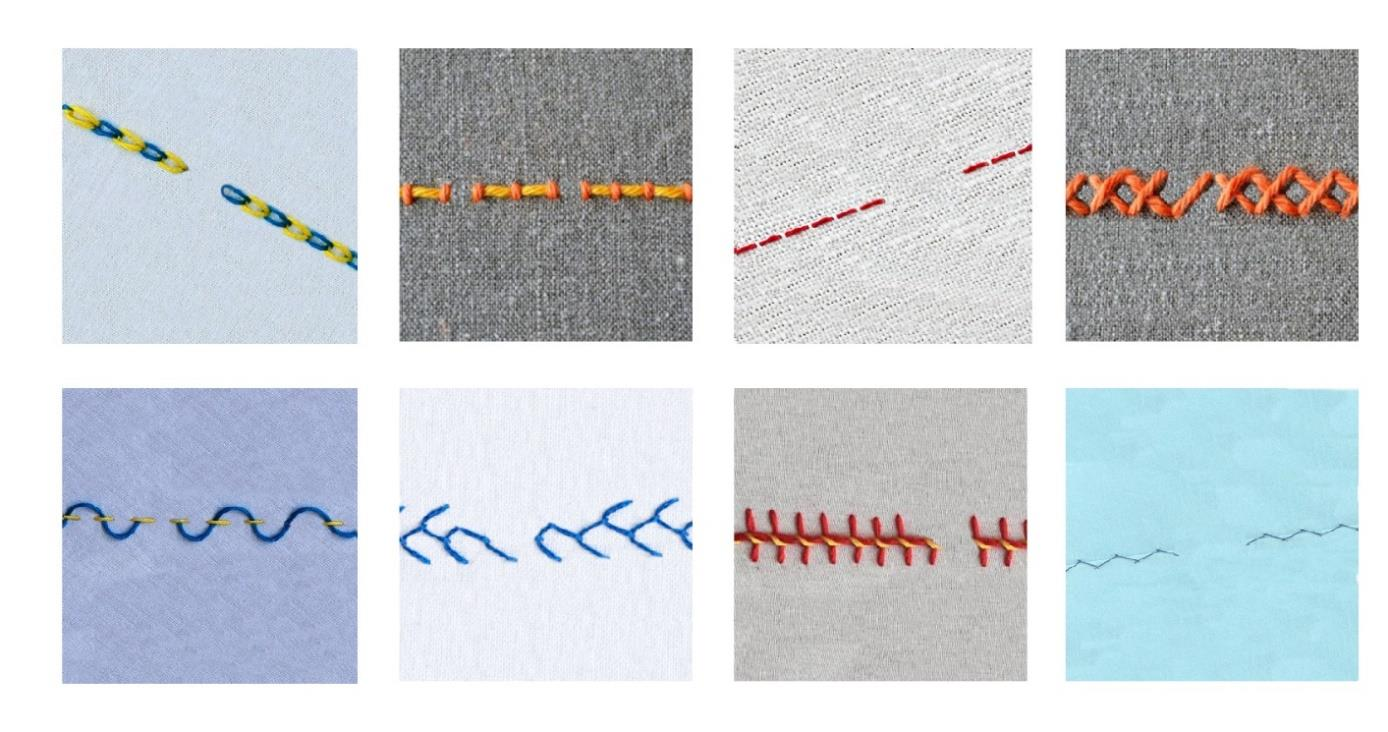
\includegraphics[width=\linewidth]{figures/page33_image2.jpeg}\\[-1mm]{\scriptsize (b) Digitally constructed defect}\end{minipage}
\caption{Historical thesis examples; (b) must not be interpreted as a naturally occurring production defect. Image reuse rights require author review.}\label{fig:examples}
\end{figure}

\subsection{Two levels of source lineage}
Each filename includes a base identifier and a UUID-like augmentation suffix. After stripping the suffix, 182 candidate image families remain: 31 \texttt{actual\_original\_XX} and 151 \texttt{faulty\_original\_XXN}. Each of the 182 family identifiers occurs in at least two original folder partitions. Accordingly, \emph{every one} of the 7,365 images belongs to an image family spread across original train/validation/test folders. There are zero identical-byte SHA-256 image groups, demonstrating why exact-byte deduplication alone does not detect transformed derivatives.

At a second, more conservative level, the filename pattern \texttt{faulty\_original\_XXN} points to \texttt{actual\_original\_XX}. All 151 faulty families syntactically map to one of the 31 normal photo candidates; automated visual similarity ranks support multiple matching pairs. This is evidence for an \emph{inferred} 31-parent graph, not proof of the original camera photographs or Photoshop edit chains. A single physical seam may also have been photographed several times, making even 31 an upper bound on reliably distinct physical sources without manual verification.

\subsection{Evaluation partitions and provenance controls}
The original train/validation/test folder membership is rejected for independent evaluation. Rather than relying on the number of JPEG/PNG records, the relevant unit of independence is the source photograph (and potentially the physical garment). A fixed random seed (20261018) groups the 31 inferred photo parents into 21 training, five validation and five internal holdout parent IDs, excluding one corrupt image. The resulting 7,364 valid images are: 5,019 training (1,878 normal, 3,141 faulty), 1,259 validation (433/826) and 1,086 holdout (422/664). No inferred photo-parent key crosses these new partitions. Nonetheless, group independence is conditional on the unverified filename-to-real-photo relation. Checkpoints, ZIP digests and partition hashes are recorded before the holdout is unsealed. The holdout workflow verifies the frozen checkpoint SHA-256, original archive checksum and manifest fingerprint, and refuses to refit models or alter the decision threshold.

\section{Models and Experiments}
\subsection{Reconstructed scratch CNN}
The new PyTorch SmallCNN reconstructs an experimental model \emph{family}, not the exact 2022 TensorFlow/Keras weights. An exploratory initial run used the \emph{older} 182-family grouping, input resolution $100\times100$, class-weighted cross entropy, Adam ($10^{-3}$), batch size 32, train-time augmentation and selection by validation macro-F1 over three completed epochs. Its 1,077-image candidate-family holdout returned 57.38\% accuracy and zero recall for normal stitches. This failure is retained as a software-verified diagnostic, not a comparable result for the subsequent 31-photo grouping.

\subsection{ImageNet-pretrained MobileNetV3-Small}
Two \emph{distinct}, fixed MobileNetV3-Small experiments~\cite{mobilenet} use ImageNet1K-V1 pretrained \emph{frozen} convolutional features with $224\times224$ RGB input, ImageNet normalization, global spatial averaging and a standardized balanced logistic regression classifier ($C=1$). The class decision threshold is 0.5; no hyperparameter sweep was carried out. The first run used the older 182-family split (5,167 training and 1,120 validation images). Its validation macro-F1 was 0.648; no holdout result from that run is claimed in this paper. The second used the inferred 31-photo-parent grouping (5,019 training, 1,259 validation); this second model alone is evaluated on the first-time 1,086-image internal parent holdout. They have different fitted heads and manifests, and must not be treated as the same model.

\subsection{First external test and separation of evidence}
Before inspecting the real StitchingNet test metrics, the \emph{older} 182-family-trained MobileNet and SmallCNN checkpoints and threshold were frozen. The official StitchingNet archive checksum was checked; for the binary task, only normal class 00 ($n=2{,}436$) and broken-stitch class 02 ($n=1{,}201$) were retained. The nine other defect classes were excluded. No external training, calibration or score-based selection was performed. Byte-identical overlap with the original ZIP was not detected, although transformed/semantic overlap cannot be excluded from hash checking alone. StitchingNet was examined \emph{once} in this protocol; later tuning cannot reuse it as an untouched external benchmark. The \emph{new} 31-photo-parent MobileNet has \emph{never} been evaluated on StitchingNet.

\section{Results and Discussion}
\subsection{Original-split audit}
The original archive's systematic cross-partition sharing of \emph{all} 182 augmentation families invalidates any assertion that its existing folders measure independent-image-family generalization. This finding does not prove the historical 94.91\% validation result used exactly the recovered folders, because its complete training scripts and run manifests are unavailable. The historical accuracy is therefore a source-reported number, not a reproduced result that can be directly subtracted from our new measurements.

\subsection{Frozen grouped internal test}
Table~\ref{tab:internal} shows the first, fixed 31-inferred-parent MobileNet holdout. Accuracy is 80.20\%, macro-F1 is 0.799, balanced accuracy is 81.74\%, and faulty recall is 74.85\%. Thus 167 of 664 edited faulty samples are missed, even before authentic broken-stitch acquisition is tested. The held-out set represents just \emph{five inferred photo parents}, so image-level sample size does not imply 1,086 statistically independent observations.

\begin{table}[!t]\centering
\caption{First frozen \emph{inferred}-photo-parent holdout (new MobileNet model; 1,086 augmented images, 5 parent candidates).}\label{tab:internal}
\setlength{\tabcolsep}{3pt}\footnotesize
\begin{tabular}{l r@{\hspace{7pt}}l r}\toprule
Metric & Value & Metric & Value\\\midrule
Accuracy & 0.8020 & Macro-F1 & 0.7995\\
Balanced acc. & 0.8174 & ROC-AUC & 0.9135\\
Normal recall & 0.8863 & Faulty recall & 0.7485\\
Normal $n$ & 422 & Faulty $n$ & 664\\\bottomrule
\end{tabular}\\[1mm]
\scriptsize Confusion matrix, rows/columns normal--faulty: $\left[\begin{smallmatrix}374&48\\167&497\end{smallmatrix}\right]$.
\end{table}

\begin{table}[!t]\centering
\caption{Variation across the five \emph{inferred} photographic parents in the first frozen internal holdout (fixed threshold).}\label{tab:parents}
\setlength{\tabcolsep}{3.2pt}\footnotesize
\begin{tabular}{lrrrrrr}\toprule
Parent & $N$ & Normal & Faulty & FP & FN & Acc.\\\midrule
AG & 213 & 89 & 124 & 3 & 8 & 94.84\\
AK & 333 & 76 & 257 & 13 & 94 & 67.87\\
AY & 245 & 99 & 146 & 13 & 36 & 80.00\\
AZ & 66 & 66 & 0 & 0 & 0 & 100.0\\
BB & 229 & 92 & 137 & 19 & 29 & 79.04\\\bottomrule
\end{tabular}
\end{table}

The five inferred parents are not equally difficult. For photo candidate \texttt{AK}, the model misses 94 of 257 faulty images, while \texttt{AG} has 8 missed faults among 124. Candidate \texttt{AZ} contains 66 normal images and \emph{no} faulty example. This heterogeneous parent-level structure limits the interpretation of the aggregate score and prevents a claim of stable accuracy across fabrics or production conditions. The holdout is now inspected: any future model revision influenced by it requires new test photos.

\subsection{First zero-adaptation StitchingNet transfer}
Table~\ref{tab:external} concerns the two \emph{earlier 182-family-trained} models only. Pretrained features substantially improve macro-F1 over the scratch CNN under domain shift, yet the MobileNet misses 507 of 1,201 genuine broken stitches. Its 66.46\% accuracy is even slightly below the 66.98\% achieved by classifying every external image as normal. Macro-F1 and class-wise recall, not accuracy alone, better describe operational usefulness. We do \emph{not} attribute the StitchingNet score to the later 31-photo-parent-trained checkpoint.

\begin{table}[!t]\centering
\caption{First frozen external test: StitchingNet 3,637 images (\emph{older 182-family models}, no external fitting).}\label{tab:external}
\setlength{\tabcolsep}{2.3pt}\footnotesize
\begin{tabular}{lrr}\toprule
Metric & Scratch CNN & Frozen MobileNet\\\midrule
Accuracy & 0.3561 & 0.6646\\
Balanced accuracy & 0.4969 & 0.6426\\
Macro-F1 & 0.3146 & 0.6354\\
Normal recall & 0.0821 & 0.7073\\
Broken recall & 0.9117 & 0.5779\\
Broken ROC-AUC & 0.4821 & 0.6874\\\bottomrule
\end{tabular}\\[1mm]
\scriptsize MobileNet confusion matrix $\left[\begin{smallmatrix}1723&713\\507&694\end{smallmatrix}\right]$; rows/columns normal--broken.
\end{table}

\subsection{Implications for garment inspection}
Both evaluations show the importance of making \emph{false negatives} visible. Internal synthetic holdout performance cannot establish production deployment quality; external real broken-stitch recall of 57.79\% is also insufficient for unattended inspection. The main contribution is transparent evidence accounting: family-level overlap in the original partitions, a reproducible inferred-parent split, and an external model comparison that is appropriately separated from later training. This is a methodologically informative negative result, not a claim that the technique outperforms recent defect-localization systems.


\subsection{Distinct error modes and aggregation effects}
The small number of source-photo candidates changes how these performance measures should be read. Consider two hypothetical operating points with the same overall accuracy but different sensitivities: one may minimize unnecessary reinspection of intact garments, while the other misses a greater fraction of structurally broken seams. At the fixed 0.5 threshold in our initial internal holdout, the model flags 48 of 422 normal images as faulty and marks 167 of 664 Photoshop-faulty images as normal. The latter error is more consequential for unattended quality inspection. There is no evidence that a different threshold would improve the real-fault trade-off on independent production images; threshold selection on the now-inspected test would invalidate its role as a frozen holdout.

An independent-seeming count of 1,086 augmented images also understates sampling correlation. Every held-out record is associated with one of just five inferred photographed sources, many derivatives of a source appearing repeatedly. Therefore an image-wise bootstrap or conventional binomial interval would likely overstate precision. Even computing a parent-level interval is difficult with only five clusters, including one all-normal source. We instead report the full per-parent confusion counts and refrain from estimating a narrow population accuracy interval. A future prospective experiment should sample many physically different garments, seams and camera acquisition sessions and should keep images of one garment together.

The ROC-AUC of 0.914 in the grouped internal set characterizes ranking over synthetic/augmented examples, not detection at the operational threshold or performance on naturally broken seams. It cannot negate the observed 25.15\% false-negative proportion for the faulty internal class. The older MobileNet's external ROC-AUC of 0.687 likewise does not negate its 42.21\% broken-seam miss proportion. The original 94.91\% historical validation number is not directly comparable with either of these values: it concerns a different and not fully reconstructed configuration, evaluation history, and possibly different partitions.

\subsection{Reproducibility controls and unperformed claims}
To preserve the two distinct model lineages, experiment outputs were archived separately. The source ZIP is identified by SHA-256 \texttt{e7aed1355a712c14bb\ldots}; the inferred-parent MobileNet holdout checkpoint by \texttt{02fa682d0648aa2521\ldots}; and its split manifest by \texttt{769d10dc6f6651f2\ldots}. The frozen evaluation verifies the full digests, class mapping and fixed threshold before reading the holdout. The training workflow for the second MobileNet never loads StitchingNet; consequently there is \emph{no} independent external performance estimate for that second model. Meanwhile the external evaluation used only models frozen \emph{before} StitchingNet performance was examined. Once a benchmark has been inspected, exploratory reuse cannot be described as another untouched test.

\subsection{Evidence still required for prospective deployment}
A new real-world evaluation must record the true physical-seam or garment identifier, original photographic file, camera, lighting, textile/thread combination, whether the defect was physically present, and independent expert review of each defect label. Photoshop-created positives should be marked separately rather than mixed with authentic positives. At least two reviewers should resolve label disputes blind to predicted class, with image and source records retained subject to owner consent. This would allow genuinely unseen source groups, per-fabric sensitivity estimates, prevalence-aware precision, confidence intervals clustered by garment, and a credible assessment of whether broken-stitch recall is high enough for a human-in-the-loop production setting. Until such data exist, the present scores are evidence about reproducibility and failure modes, not certification of a factory inspection product.

\section{Limitations and Conclusion}
Original unedited photographs, Photoshop edit histories, and per-image ownership/source logs are missing. The syntactic 151-to-31 parent mapping is supported by filenames and visual similarity but remains unconfirmed by the original image creators. The number of truly distinct garment sources may be smaller than 31. The 7,364 readable images contain synthetic defects and transformations; only five inferred parents entered the internal test. Results are sensitive to parent composition, labels, domain shift, camera setup and a single experiment seed. The original 2022 record also contains inconsistent augmented-image counts and does not preserve the run needed to reproduce its published validation score. We have not performed a new independently sourced real broken-seam test for the later 31-photo-parent checkpoint; public derivative releases of StitchingNet are not a second independent dataset.

In conclusion, this audit demonstrates that \emph{all 182 augmentation families} in the recovered source ZIP cross original partitions. After inferred-photo-parent grouping, a pretrained MobileNet classifier scores 0.799 macro-F1 on a small augmented-image holdout, whereas an \emph{earlier} pretrained model yields 0.635 macro-F1 with 57.79\% defect recall on previously unseen real StitchingNet images. These experiments demonstrate the importance of provenance-aware splitting and honest external metrics, but they do not validate photo-source independence or operational reliability. The next necessary evidence is human confirmation of original photo/edit lineage and a new, separately acquired, expertly labelled collection of genuinely broken sewn seams.

\section*{Generative-AI Use Disclosure}
ChatGPT assisted with literature exploration, research software and experiment workflow design, manuscript drafting and LaTeX editing. Numerical metrics reproduced here were generated by archived, executable GitHub Actions runs rather than invented. The human authors are responsible for checking source provenance, interpretations, originality, citations, data permissions and conference rules before submission.

\begin{thebibliography}{00}
\bibitem{ngan} H. Y. T. Ngan, G. K. H. Pang, and N. H. C. Yung, ``Automated fabric defect detection---A review,'' \emph{Image Vis. Comput.}, vol. 29, no. 7, pp. 442--458, 2011, doi: 10.1016/j.imavis.2011.02.002.
\bibitem{kim} H. Kim \emph{et al.}, ``Broken stitch detection method for sewing operation using CNN feature map and image-processing techniques,'' \emph{Expert Syst. Appl.}, vol. 188, art. 116014, 2022, doi: 10.1016/j.eswa.2021.116014.
\bibitem{chowdhury} H. Chowdhury \emph{et al.}, ``Broken stitch detection method for sewing operation using deep learning,'' in \emph{Proc. Int. Conf. Innovations in Science, Engineering and Technology (ICISET)}, 2024, doi: 10.1109/ICISET62123.2024.10939324.
\bibitem{stitchingnet} W.-K. Jung, J. Kang, W. Kwon, and H. Kim, ``StitchingNet and deep transfer learning method for sewing stitch defect detection,'' \emph{J. Comput. Des. Eng.}, vol. 12, no. 4, pp. 140--154, 2025, doi: 10.1093/jcde/qwaf037.
\bibitem{patchcore2026} J. Kim \emph{et al.}, ``An efficient anomaly detection method for the industrial sewing process using PatchCore and fine-tuned ResNet,'' \emph{Sci. Rep.}, 2026, doi: 10.1038/s41598-026-73203-5.
\bibitem{stitchingnetseg2026} J. Park, W.-K. Jung, and H. Kim, ``StitchingNet-Seg: a semantic segmentation dataset of industrial sewing stitch defects,'' \emph{Sci. Data}, 2026, doi: 10.1038/s41597-026-08496-2.
\bibitem{mobilenet} A. Howard \emph{et al.}, ``Searching for MobileNetV3,'' in \emph{Proc. IEEE/CVF Int. Conf. Comput. Vis.}, 2019, pp. 1314--1324.
\end{thebibliography}
\end{document}